\section{Problem 4}
State space representation with input derivatives.

For the following mechanical system, input is the displacement $u$ and output is the displacement $z$.

\begin{figure}[htp]
    \centering
    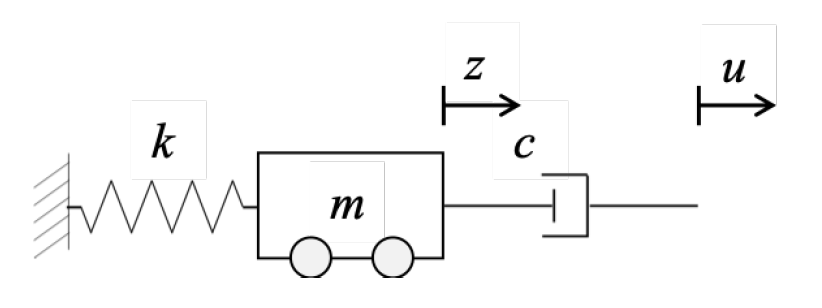
\includegraphics[width=6cm]{images/Q4.png}
\end{figure}

\subsection{a)}
Find the state space representation of this system.
\subsubsection{\textit{ Sol. }}

Draw FBD to analyze system dynamics: 
\begin{figure}[htp]
    \centering
    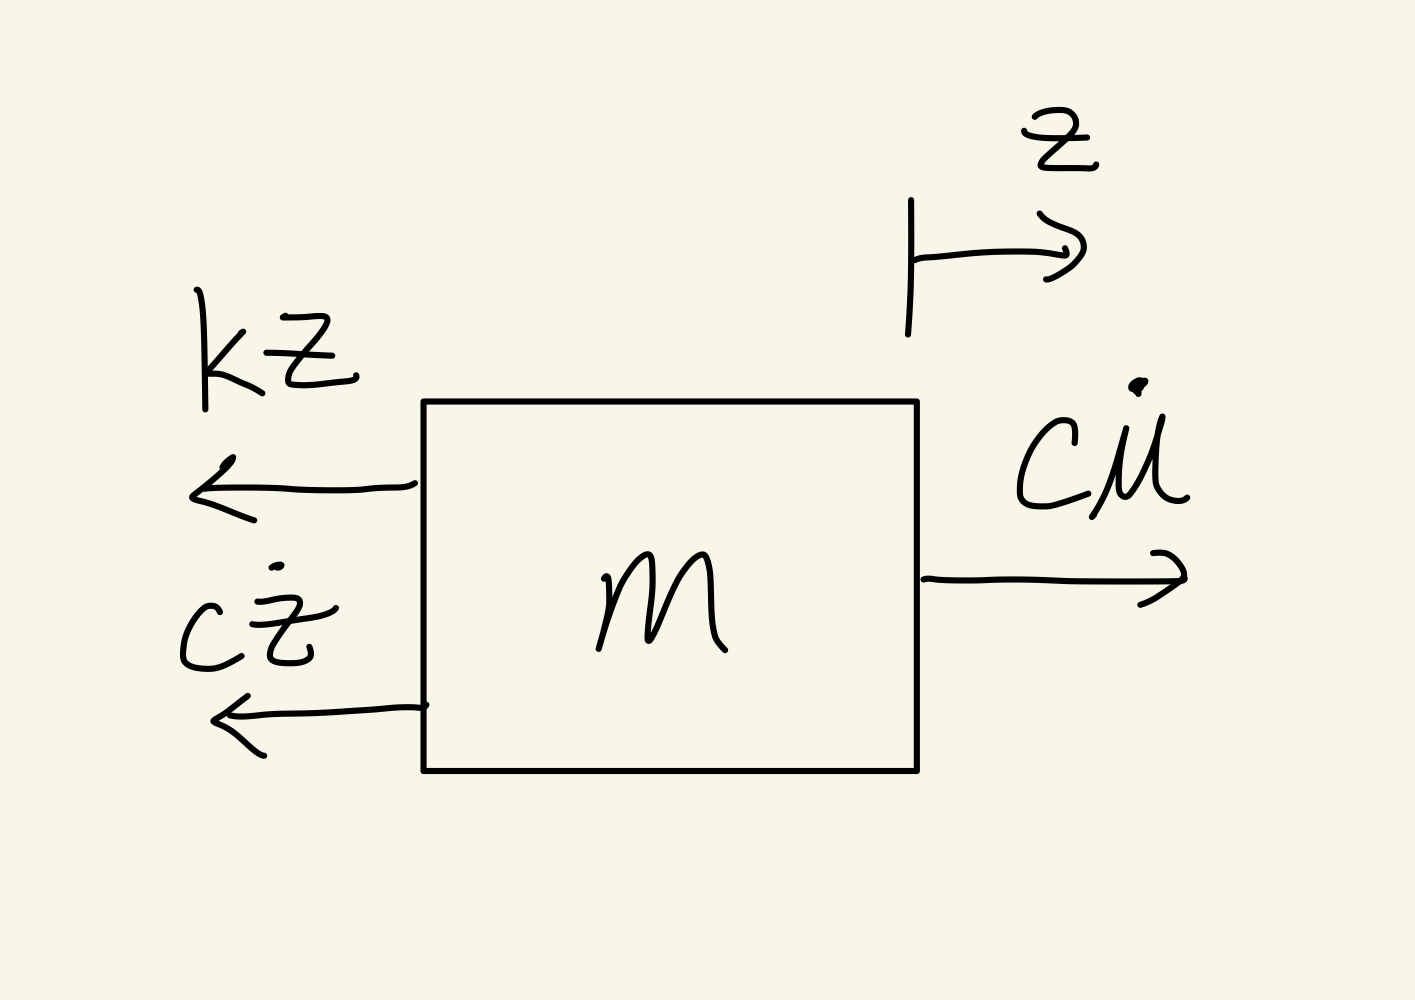
\includegraphics[width=6cm]{images/Q4_FBD.png}
    \caption{Free body diagram}
    \label{fig:Q4FBD}
\end{figure}

We get the following dynamic equation: $m\ddot{z} = -kz-c\dot{z}+c\dot{u}$ $\Rightarrow$ $\ddot{z} = -\frac{k}{m}z-\frac{c}{m}\dot{z}+\frac{c}{m}\dot{u}$

Because we have derivative of input, we can define the state vector as: $\textbf{x} = 
\begin{bmatrix}
    x_1\\
    x_2
\end{bmatrix} = 
\begin{bmatrix}
    z\\
    \dot{z} - \frac{c}{m}u
\end{bmatrix}$, and output $y = z$.

From $\ddot{z} = -\frac{k}{m}z-\frac{c}{m}\dot{z}+\frac{c}{m}\dot{u}$ 

$\Rightarrow$     
$\left\{
    \begin{array}{lr}
    \dot{x_1} = \dot{z} = \left(\dot{z} - \frac{c}{m}u\right) +  \frac{c}{m}u = x_2 + \frac{c}{m}u\\
    \dot{x_2} = \ddot{z} - \frac{c}{m}\dot{u} = -\frac{k}{m}z-\frac{c}{m}\dot{z}+\frac{c}{m}\dot{u} - \frac{c}{m}\dot{u} = -\frac{k}{m}z - \frac{c}{m}(x_2 + \frac{c}{m}u) = -\frac{k}{m}x_1 - \frac{c}{m}x_2 - \left(\frac{c}{m}\right)^2u
    \end{array}
\right.$ 

We get: 
\begin{equation}
    \begin{aligned}
        \dot{\textbf{x}} &=
        \begin{bmatrix}
            0 & 1 \\
            -\frac{k}{m} & -\frac{c}{m}
        \end{bmatrix}
        \textbf{x} + 
        \begin{bmatrix}
            \frac{c}{m}\\
            -\left(\frac{c}{m}\right)^2
        \end{bmatrix}
        u
        \\
        y &=
        \begin{bmatrix}
            1 & 0
        \end{bmatrix}
        \textbf{x} + 
        \begin{bmatrix}
            0
        \end{bmatrix}
        u
    \end{aligned}
\end{equation}
\subsection{b)}
Assume that $m =10 kg$, $c =20 N-s/m$, $k =40 N/m$, and the input displacement is a step displacement of $0.2 m$. Use Matlab to plot the response $z(t)$. Include your code and plot. Is there anything unusual about this step response? Why is this the case for this system?

Matlab code:
    \lstinputlisting{codes/Question4b.m}
Result:
\begin{figure}[htp]
    \centering
    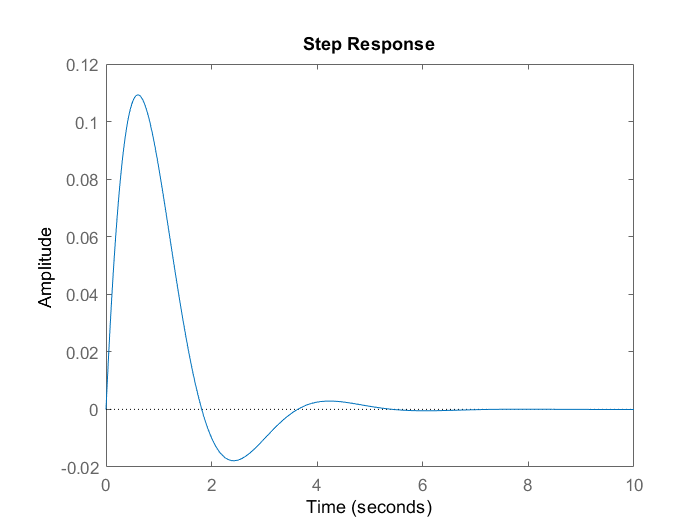
\includegraphics[width=12cm]{images/Q4_b_fig.png}
    \caption{Step Response}
    \label{fig:Q4b}
\end{figure}

The step response is as expected. The final value goes to zero, because the first derivative of the input $u$ only changes at time $0_{+}$, thus energy is added to the system only at time $0_{+}$. And because this is a damped system, total energy in the system will eventually dissipate to zero.
\pagebreak